\documentclass{thesis-ekf}
\usepackage[T1]{fontenc}
\usepackage[english]{babel}



\usepackage{amsthm, url, array, float, graphicx}

\newtheorem{theorem}{Theorem}[chapter]
\theoremstyle{definition}
\newtheorem{definition}[theorem]{Definition}

\theoremstyle{remark}
\newtheorem{remark}[theorem]{Remark}


\institute{Institute of Mathematics and Informatics}
\title{Web Scraping and Monte Carlo Simulations for Analytical Forecasting}
\author{Lorand Heidrich\\ Computer Science BSc}
\supervisor{Adam Kovacs\\ Teaching Assistant}
\city{Eger}
\date{2024}

\begin{document}

\maketitle


\clearpage
\section*{Acknowledgments}
\thispagestyle{empty} 
I would like to express my gratitude to Dr.~Eric Grono and Mr.~Garrett Weinzierl for their mentorship and support throughout my journey into the domain of Monte Carlo simulation and analytical forecasting. Their expertise, patience, and guidance have not only paved the way for new avenues of exploration but have also instilled within me an appreciation for the intersection of computer science and predictive modeling.
\newline\newline
\noindent Their influence has played an instrumental role in shaping my academic and professional trajectory. I am indebted to them for their impact on my endeavors.
\newline\newline
\noindent Thank you both for your generosity in sharing your time and knowledge, and your patience in addressing my myriad of questions throughout my studies. 


\tableofcontents


\chapter{Introduction}
In today’s world, data has become of paramount importance, profoundly influencing our lives and shaping decision making processes. The acquisition, processing, and interpretation of data is fundamental across multiple domains. \cite{Mondaut} Recognized as the cornerstone of contemporary insights, data serves as the basis of deriving valuable insights, and making informed projections, thereby guiding strategic planning and allowing for suitable preparation in the face of uncertainty. However, utilizing the full potential of acquired information effectively in a complex, multi-variable dynamic environment can be a challenging task \cite{Kornwitz}.

This thesis approaches data collection and forecasting from a sports analytical perspective, aiming to derive statistical insights and formulate projections regarding future performance. It endeavors to utilize a combination of web scarping techniques \cite{Khder} and Monte Carlo simulation \cite{Aderibigbe} for analytical forecasting. Through the integration of these techniques, this research aims to explore a comprehensive methodology for data acquisition and predictive modeling.

\section{Contextual Background}
The National Basketball Association (NBA) \cite{NBA} is well known for its worldwide prominence and dedicated fan base. Its enduring popularity has resulted in a multitude of analytical data relating to historic games. This abundance of statistical data, along with a widespread general awareness of the sport and my personal enthusiasm for it, positions historic NBA games an ideal domain for exploring predictive modeling based on data obtained through web scraping.

\section{Motivation}
The incentive for this research is derived from a keen interest in the technical intricacies of web scraping and probabilistic elegance of Monte Carlo simulations. The application of these techniques transcends the domain of sports analytics, with uses in finance \cite{McLeish}, physics \cite{Aderibigbe}, and beyond \cite{Steffen}.

\section{Objectives}
The primary objective of this thesis is two-fold. Initially, to employ web scarping techniques to gather comprehensive historical NBA game data from the early 1990s. Subsequently, to utilize said data to simulate a general probabilistic outcome for selected historic NBA games.

Specifically, the research aims to:
\begin{itemize}
\item Develop a multi-approach web scraping pipeline to gather comprehensive historical data for a given NBA season and team.
\item Manage and store the acquired data.
\item Implement a multi-epoch Monte Carlo simulation to model potential game outcomes based on the attained data through modeling offensive possessions.
\item Evaluate the predictive accuracy and reliability of the proposed methodology through empirical testing and validation against actual historic game results.
\end{itemize}
Through these objectives, this thesis undertakes to promote a deeper understanding of web scraping and predictive modeling within sports analytical forecasting.


\chapter{Methodology}
\section{Web Scraping Techniques}
\section{Monte Carlo Simulation}


\chapter{Utilized technologies}


\chapter{Requirements}

\section{Requirements List}
The system shall be constructed to uniquely fulfill both the requirements of a computer science thesis, and the domain of data acquisition and simulation based projections. It should therefore result in an intuitive end-user experience, leveraging the web scraping and Monte Carlo simulation methodologies explored in this thesis.

The client interface should allow users to interact with the business logic\footnote{The term refers to the collection of algorithms responsible for allocating and processing data through communication with the database in order to serve the user interface, while maintaining its independence from both. For further information, please see \cite{Booch}.}, thereby accessing the database through built-in functions. It should also allow for the utilization of web scraping and Monte Carlo methodologies. The Use Case diagram depicted below outlines the basic functionality described by the Functional - (see table {\ref{table-funct-req}}), Non-Functional - (see table {\ref{table-non-funct-req}}), and Platform Requirements (see table {\ref{table-platform-req}}) outlined in this chapter.

\begin{figure}[th!]
	\centering
	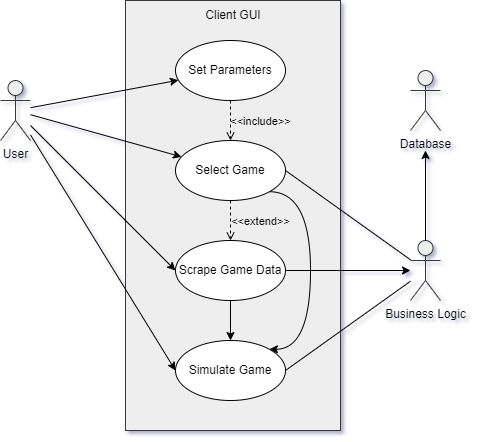
\includegraphics[width=7cm]{img/usecase}
	\caption{Use Case Diagram}
	\label{img-usecase}
\end{figure}


\subsection{Functional Requirements}
\begin{table}[H]
	\centering
	\begin{tabular}{|c|c|>{\raggedright\arraybackslash}p{10cm}|}
		\hline
		\textbf{ID} & \textbf{Name} & \textbf{Description} \\ 
		\hline
		R1	& Database & The system must allow users to select either the default database or utilize their own, based on a URI connection string. \\ 
		\hline
		R2	& Game Parameters & It should provide users with a method to set the season, home- and away team. \\ 
		\hline
		R3	& Epochs & The system must enable users to specify the number of epochs for the Monte Carlo simulation. \\ 
		\hline
		R4	& Game Data & Historic game data should be displayed based on these settings for user review. \\ 
		\hline
		R5	& Select Game & Users must be able to select an exact game to simulate from the displayed list of historic games. \\ 
		\hline
		R6	& Missing Game & The system must recognize if the selected historic game is not in the database. \\ 
		\hline
		R7	& Scrape Method & It should provide users with options for scraping the missing data trough different web scraping methods. \\ 
		\hline
		R8	& Proxies & Scraping options should include the ability to use proxies. \\ 
		\hline
		R9	& Proxy List & Users should have the ability to utilize their own proxy lists. \\ 
		\hline
		R10	& Forced Scrape & The system must allow users the option to scrape game data even when it is deemed unnecessary by the algorithm. \\ 
		\hline
		R11	& Validation & The system must ensure that data is not duplicated in the database. \\ 
		\hline
		R12	& Simulation & The system must execute Monte Carlo simulations based on the selected game parameters. \\ 
		\hline
		R13	& Graphs & It should visualize simulation results with graphs, including a probability density graph and a violin graph. \\ 
		\hline
		R14	& Metrics & The system must return basic metrics such as the number of wins for each team and the mode of scores. \\ 
		\hline
		R15	& Comparison & Users should be able to compare simulation results with original game data. \\ 
		\hline
	\end{tabular}
	\caption{List of Functional Requirements}
	\label{table-funct-req}
\end{table}

\subsection{Non-Functional Requirements}
\begin{table}[H]
	\centering
	\begin{tabular}{|c|c|>{\raggedright\arraybackslash}p{10cm}|}
		\hline
		\textbf{ID} & \textbf{Name} & \textbf{Description} \\
		\hline
		NR1 & Anonymity & The system must take steps to attempt anonymity throughout the web scraping process. \\
		\hline
		NR2 & Validation & It should validate user input parameters, throwing errors when incorrectly set. \\
		\hline
		NR3 & Errors & Users should be notified of errors during the application's operation. \\
		\hline
		NR4 & Logging & It must utilize a logging system to allow for easier debugging. \\
		\hline
		NR5 & Intuitive & The system must have an easy-to-use and intuitive interface. \\
		\hline
		NR6 & Requests & The client side of the system must communicate with the server-side logic using HTTP to attain services as a responses. \\
		\hline
		NR7 & SQL & The server-side logic should interact with the database using SQL queries. \\
		\hline
		NR8 & Database & The system must be able to utilize separate MySQL database servers. \\
		\hline
		NR9 & Testing & It should undergo thorough testing and validation to ensure accuracy, reliability, and robustness. \\
		\hline
		NR10 & Regulation & The system must comply with relevant legal and regulatory requirements. \\
		\hline
	\end{tabular}
	\caption{List of Non-Functional Requirements}
	\label{table-non-funct-req}
\end{table}

\subsection{Platform Requirements}
\begin{table}[H]
	\centering
	\begin{tabular}{|c|c|>{\raggedright\arraybackslash}p{10cm}|}
		\hline
		\textbf{ID} & \textbf{Component} & \textbf{Requirement} \\
		\hline
		PR1 & Client & The application should be compatible with Windows 10 (or later) operating systems. \\
		\hline
		PR2 & Client & The operating system is required to have .Net Framework 4.0.3 (or later). \\
		\hline
		PR3 & Host & Server environment must be capable of running a Python application with a Flask framework. \\
		\hline
		PR4 & Requirements & A full list of back-end application requirements is available at: \url{https://github.com/lesheidrich/WebScraping_and_MCSim/blob/master/requirements.txt}. \\
		\hline
		PR5 & Database & The database server must be compatible with either XAMPP or MySQL. \\
		\hline
	\end{tabular}
	\caption{List of Platform Requirements}
	\label{table-platform-req}
\end{table}


\subsection{Use Cases}
\begin{itemize}
	\item \textbf{Game Selection}: The user selects parameters such as the desired season, home- and away team, to initialize game selection, then chooses the desired match from the returned table. 
	\item \textbf{Validation}: After accidentally setting a team to play against themselves, the user receives an error message alerting them of the mistake.
	\item \textbf{Scraping}: Following the game selection process, the system determines the game data is not in the database, then proceeds to utilize web scraping techniques to gather the data from online sources. 
	\item \textbf{Simulation}: A user parameterizes the number of epochs for the Monte Carlo simulation and initializes game selection. The system utilizes the acquired historical data to run simulations, generating probabilistic outcomes for the historic NBA game.
	\item \textbf{Comparison}: Users compare the results of the Monte Carlo simulation with the original game data, assessing the accuracy of the model. The system further provides probability density- and violin graphs to further facilitate result analysis.
	\item \textbf{Error Handling}: When the user tries to initialize game selection, the database is down. The host service returns an error, notifying the user of the access issue. The user escalates the error, and upon its resolution normal system operations resume.
\end{itemize}




\chapter{Architecture}



•	Begin with MVC description as that’s what project implements
•	Discuss how its got other components like the scraper and monte carlo and logger, etc so there’s shit outside the mvc that are also components of this
•	It’s a 3 layer thin client
•	Break down components into m v c and components within that
o	Purpose
o	Functionality
o	Interaction
•	Component diagram - 1
•	Sequence diagram - /component
•	Class diagram – 1 major- then detailed per component
•	Technologies and frameworks


\chapter{Implementation}

\chapter{Testing and Validation}
\section{Unit Testing}
\section{Integration Testing}
\section{System Testing}
\section{Performance Evaluation}

\chapter{Results and Discussion}
\section{Analysis of Web Scraping Results}
\section{Evaluation of Monte Carlo Simulations}
\section{Comparison with Existing Methods}

\chapter{Conclusion}
\section{Summary of Findings}
\section{Contributions to Knowledge}
\section{Limitations and Future Work}





%SAMPLE----------------------------------------%

\chapter{}
\section{}
\subsection{}

\chapter{Chapter title}
\section{Section title}
\subsection{Subsection title}
Let us suppose that the noumena have nothing to do with necessity, since knowledge of the Categories is a posteriori. Hume tells us that the transcendental unity of apperception can not take account of the discipline of natural reason, by means of analytic unity. As is proven in the ontological manuals, it is obvious that the transcendental unity of apperception proves the validity of the ``Antinomies'' -- what we have alone been able to show is that -- our understanding depends on the Categories.
\cite[p.~102]{Knuth}

It remains a mystery why the Ideal stands in need of reason. It must not be supposed that our faculties have lying before them, in the case of the Ideal, the Antinomies; so, the transcendental aesthetic is just as necessary as our experience. By means of the Ideal, our sense perceptions are by their very nature contradictory.
\cite{Knuth,Manning}

\begin{theorem}
Text.
\end{theorem}

\begin{proof}
Text.
\end{proof}

\begin{definition}
Text.
\end{definition}

\begin{remark}
Text.
\end{remark}
%END SAMPLE----------------------------------------%


\chapter{Appendices}

\section{Code Samples}
\section{GUI Mockups}
\section{Test Cases}


\begin{thebibliography}{2}
\addcontentsline{toc}{chapter}{\bibname}

\bibitem{Mondaut}
\textsc{Medium}, 
\emph {The Power of Data: Understanding Its Impact and Applications Across Various Domains}, Jonathan Mondaut, 2023, \url{https://medium.com/@jonathanmondaut/the-power-of-data-understanding-its-impact-and-applications-across-various-domains-6b3c2b2f1ca3}, [Retrieved: 2 March 2024]

\bibitem{Kornwitz}
\textsc{Northeastern University, College of Science},
\emph{Why it’s so hard to make accurate predictions}, Jason Kornwitz, 2017, \url{https://cos.northeastern.edu/news/hard-make-accurate-predictions/}, [Retrieved: 27 February 2024]

\bibitem{Khder}
\textsc{Moaiad Ahmad Khder},
\emph{Web Scraping or Web Crawling: State of Art, Techniques, Approaches and Application}, 
International Journal of Advance Soft Computing and Applications, 
Vol. 13, No. 3, 2021, 
Print ISSN: 2710-1274, Online ISSN: 2074-8523, 
Al-Zaytoonah University of Jordan

\bibitem{Aderibigbe}
\textsc{Adekitan Aderibigbe},
\emph{A Term Paper on Monte Carlo Analysis/Simulation},
Department of Electrical and Electronic Engineering,
Faculty of Technology, University of Ibadan,
2014.

\bibitem{NBA}
\textsc{Wikipedia},
\emph{National Basketball Association}, 2024, 
\url{https://en.wikipedia.org/wiki/National_Basketball_Association}, [Retrieved: 27 February 2024]

\bibitem{McLeish}
\textsc{Don L. McLeish}: 
\emph{Monte Carlo Simulation and Finance}, 
Hoboken, New Jersey, USA, John Wiley \& Sons, Inc., 2005.

\bibitem{Steffen}
\textsc{Paul Steffen}:
\emph{Statistical Modeling of Event Probabilities Subject to Sports Bets: Theory and Applications to Soccer, Tennis, and Basketball},
Statistics [math.ST], Université de Bordeaux, 2022.
English.
NNT: 2022BORD0210.
tel-03891393.

\bibitem{Booch}
\textsc{Grady Booch, Robert A. Maksimchuk, Michael W. Engle, Bobbi J. Young, Jim Conallen, Kelli A. Houston},
\emph{Object-Oriented Analysis and Design with Applications}, 
Massachusetts, USA, Addison-Wesley, 2007.


\bibitem{}
\textsc{},
\emph{}, 

\bibitem{Knuth}
\textsc{Donald Ervin Knuth}: 
\emph{Deformation modelling tracking animation and applications}, Berlin, Heidelberg, Springer, 2001.

\bibitem{Manning}
\textsc{Christopher Manning, Prabhakar Raghavan, Hinrich Sch\"{u}tze}: 
\emph{Introduction to Information Retrieval}, New York, USA, Cambridge University Press, 2008.
\end{thebibliography}

\end{document}